% This is an example of how to format a thesis with LaTeX the
% simplest possible way (permitted beginning in 2010).
% NO UGA STYLE SHEET IS NEEDED.

\documentclass[12pt]{report}
\usepackage{fullpage}
\usepackage{setspace}\doublespacing    % important!
\usepackage{graphicx}
\usepackage{cite}
\usepackage{adjustbox}
\textfloatsep 0.75in                   % important with double spacing

\begin{document}

% Make the official abstract page
\newpage
\thispagestyle{empty}
\vspace*{18pt}
\begin{center}
\textsc{Structure Forming Processes in\\Mesoscopic Polymer Systems}\\[18pt]
by\\[18pt]
\textsc{Tomas Koci}\\[12pt]
(Under the direction of Michael Bachmann)\\[12pt]
\textsc{Abstract}
\end{center}
This is going to be the best abstract ever :)

% Display the index words (this is a bit fancy):
\begin{list}{\sc Index words:\hfill}{\labelwidth 1.2in\leftmargin 1.4in\labelsep 0.2in}
\item 
\begin{flushleft}\singlespacing
Polymer Aggregation,
Monte Carlo Simulations,
Parallel Tempering,
Multicanonical Sampling,
Canonical Analysis, 
Microcanonical Inflection-Point Analysis,
Flexible Polymer,
Structural Transitions,
Finite Systems,
Finite-Size Effects
\end{flushleft}
\end{list}



% Make the official title page
\newpage
\thispagestyle{empty}
\vspace*{18pt}
\begin{center}
\textsc{Structure Forming Processes in\\Mesoscopic Polymer Systems}\\[18pt]
by\\[18pt]
\textsc{Tomas Koci}\\[12pt]
B.A., The Juilliard School, 2008\\
\vfill
A Dissertation Submitted to the Graduate Faculty \\
of The University of Georgia in Partial Fulfillment \\
of the \\
Requirements for the Degree \\[10pt]
\textsc{Doctor of Philosophy}\\[36pt]
\textsc{Athens, Georgia}\\[18pt]
2016
\end{center}

% Make the copyright page
\newpage
\thispagestyle{empty}
\vspace*{5.5in}
\begin{center}
\copyright 2016 \\
Tomas Koci \\
All Rights Reserved
\end{center}

% Make the approval page
\newpage
\thispagestyle{empty}
\vspace*{18pt}
\begin{center}
\textsc{Structure Forming Processes in\\Mesoscopic Polymer Systems}\\[18pt]
by\\[18pt]
\textsc{Tomas Koci}
\end{center}
\vfill
\begin{flushleft}\singlespacing
\hskip 200pt {Approved:}\\
\vskip 12pt
% Two major professors.  If you have only one, change word to "Professor".
\hspace*{200pt}\makebox[100pt][l]{Major Professor:}Michael Bachmann\\
\vskip 12pt
% Committee (use as many lines as needed)
\hspace*{200pt}\makebox[100pt][l]{Committee:       }Steven P. Lewis\\
\hspace*{200pt}\makebox[100pt][l]{~                }Heinz-Bernd Schuttler\\
% Approval words
\vfill
Electronic Version Approved:\\[12pt]
Alan Dorsey\\
Dean of the Graduate School\\
The University of Georgia\\
July 2016
\end{flushleft}


% Now we begin the regular LaTeX document.
% You may want to have a regular LaTeX title page here...

\chapter*{Acknowledgments}
\pagenumbering{roman}
\setcounter{page}{4}

\setcounter{tocdepth}{1}
\tableofcontents
\listoffigures  % if any
\listoftables % if any

\chapter{Introduction}
\pagenumbering{arabic}
\setcounter{page}{1}
Kickass intro...


\chapter{Elements of Statistical Mechanics}
Statistical mechanics aims at explaining the microscopic origins of macroscopic properties of systems with large numbers of degrees of freedom. The exact solution for a single phase space trajectory of a complex system requires enormous computational efforts and in most cases provides only a limited insight. In contrast to the chaotic nature of most phase space trajectories, collective system properties such as entropy, pressure, or temperature, for the most part exhibit relatively simple behavior. The formalism of statistical mechanics allows us to study these properties by considering the average behavior of a large number of identically prepared systems, i.e. the statistical ensemble. It is well established that in the thermodynamic limit all ensembles become equivalent. However this is emphatically not true in the case of intrinsically finite systems for which the choice of an ensemble is non-trivial. Therefore, I shall briefly discuss several prominent statistical ensembles starting with the most fundamental one, the \textit{microcanonical ensemble}.

\section{The microcanonical ensemble}
Let us consider a mechanically and adiabatically isolated system with a constant number of particles $(N)$, volume $(V)$, and energy $(E)$. At any given moment, the system is to be found in a particular microstate $\mu$, which is represented by a point in a $6N$ dimensional phase-space. At a fixed energy $E$, the accessible microstates are constrained to the surface of constant energy $\mathcal{H}(\mu) = E$, where $\mathcal{H}$ is the Hamiltonian of the system. The total number of microstates corresponding to a macrostate with a fixed energy $E$ is obtained by calculating the density of states\footnote{In the context of computer simulations, the energy space becomes by necessity discretized and the density of states is determined by counting the number of microstates within some finite energy range $[E,E+\Delta E]$.}\textsuperscript{,}\footnote{Please refer to section 2.3 for detailed discussion of alternative definitions of the density of states.}
\begin{equation}
g(E) = \int \mathcal{DP}\mathcal{DQ} \:\: \delta(E - \mathcal{H}(\mathcal{P},\mathcal{Q})),
\end{equation} 
where 
\begin{equation}
\mathcal{DP}\mathcal{DX} = \prod_{n = 1}^{N} \frac{d^{3}p_{n}d^{3}x_{n}}{(2 \pi \hbar)^{3}}
\end{equation}
is the Lebesgue measure over phase space.
Assuming that no additional quantities are conserved, i.e. the system is ergodic, all accessible microstates have equal a priori probabilities. The microcanonical equilibrium probability distribution is given by 
\begin{equation}
p(\mu)_{E} = \left\{
\begin{array}{lr}
1/g(E), & \quad
\mathrm{if} \: \mathcal{H(\mu)} = E\\
0, & \quad \mathrm{if} \: \mathcal{H(\mu)} \neq E,
\end{array}
\right.
\end{equation}
and the expectation value of an observable $O$ at a fixed energy $E$ is found by averaging over the surface of constant energy
\begin{equation}
\left< O \right>_{E} = \int \mathcal{DP}\mathcal{DQ} \:\: O(\mathcal{P},\mathcal{Q}) \:\: \delta(E - \mathcal{H}(\mathcal{P},\mathcal{Q})).
\end{equation}
The density of states of a typical mesoscopic system can easily span several thousands of orders of magnitude. It is therefore convenient to define the microcanonical equilibrium entropy
\begin{equation}
S(E) = k_\mathrm{B}\, \mathrm{ln}\, g(E),
\end{equation}
as an \textit{extensive} quantity with dimensions of energy over temperature.\footnote{If temperature is measured in the more natural units of energy, entropy becomes a unitless quantity and the Boltzmann constant equals to unity.}


\subsection{Microcanonical temperature}
Temperature is one of the fundamental concepts of statistical mechanics and has been traditionally defined in terms of the average kinetic energies of particles in a system. Here we motivate a more fundamental definition of temperature as an intrinsic system property, which can be obtained directly from the microcanonical density of states $g(E)$. For this purpose, let us consider an adiabatically isolated system composed of two weakly interacting subsystems, $S_{1}$ and $S_{2}$. The energy of the combined system is fixed and can be written as the sum of the energies of the two subsystems $E = E_{1} + E_{2}$. The probability density for a given pair of subsystem energies $(E_{1},E_{2})$ is  
\begin{equation}
\rho(E_{1},E_{2}) = \frac{g_{1}(E_{1})g_{2}(E-E_{1})}{g(E)},
\end{equation}
where the density of states of the combined system is expressed as a convolution
\begin{equation}
g(E) = \int dE_{1}g_{1}(E_{1})g_{2}(E-E_{1}).
\end{equation}
In systems with many degrees of freedom, the probability density $\rho(E_{1},E_{2})$ is a sharply peaked distribution around the equilibrium energies $(\bar{E}_{1},\bar{E}_{2})$\footnote{The energy fluctuations per particle around the equilibrium energy $\bar{E}_{1}$ scale as $N^{-1/2}$.}. These can be found by setting the energy derivative of the probability density to zero, from which we obtain
\begin{equation}
\frac{1}{g_{1}}\frac{dg_{1}}{dE_{1}}\bigg|_{\bar{E}_{1}} = \frac{1}{g_{2}}\frac{dg_{2}}{dE_{2}}\bigg|_{E - \bar{E}_{1}},
\end{equation}
or alternatively in terms of the microcanonical entropy
\begin{equation}
\frac{dS_{1}}{dE_1}\bigg|_{\bar{E}_{1}} = \frac{dS_{2}}{dE_{2}}\bigg|_{E - \bar{E}_{1}}.
\end{equation}
Motivated by the familiar observation that interacting systems at thermal equilibrium have equal temperatures, we define the microcanonical temperature as 
\begin{equation}
T(E) = \left(\frac{dS(E)}{dE}\right)^{-1}.
\end{equation}
Frequently, it is more convenient to consider the inverse microcanonical temperature defined as 
\begin{equation}
\beta(E) = \frac{dS(E)}{dE}.
\end{equation}
In the following section, we discuss the central role of inverse microcanonical temperature and its energy derivatives in the classification of structural phase transitions.

\subsection{Microcanonical analysis of phase transitions}
A macrostate of a system is specified by a set of macroscopic variables and possesses the characteristics of the predominant microstates. Macrostates are said to belong to the same thermodynamic phase, if in a given range of some external control parameters\footnote{Some common examples of external control parameters are the canonical temperature, pressure, or the chemical potential.} all of the system's thermodynamic observables are analytic, i.e. have convergent Taylor expansions. Singularities in the observables signify the presence of phase transitions between distinct phases, typically marked by abrupt changes in macrosopic properties in response to minute variations of external control parameters. Phase transitions can be roughly divided into two categories. \textit{Abrupt} transitions are characterized by the coexistence of two distinct phases and discontinuities in most physical properties. \textit{Continuous} transitions, although less common in nature, have been the object of most intense research. They are marked by diverging correlation lenghts, large fluctuations, and scale invariance. 

Divergences and singularities in thermodynamic observables and their derivatives are only found in systems which satisfy the thermodynamic limit. In mesoscopic systems\footnote{Typical length scales in  mesoscopic systems are of the order of $\sim 10$ nanometers. In this regime, exact quantum many-body interactions can be replaced by effective classical potentials, and cooperative effects dominate structure formation processes. Mesoscopic systems are distinct from macroscopic systems due to the presence of significant finite-size effects, which disallow the simplifying assumptions of the thermodynamic limit.}, due to finite size effects, divergences are replaced by peaks and discontinuities are smoothed over. For clarity, we designate the term \textit{pseudophase transition} to represent significant conformational changes in finite systems. Likewise, thermodynamic phases in finite systems shall be referred to as \textit{pseudophases}. In the following, we present a powerful formalism for the analysis of pseudophase transitions in the microcanonical ensemble; the microcanonical inflection point analysis.

\subsubsection{Microcanonical inflection-point analysis}
Unlike its canonical counterpart~-- the heat-bath temperature~-- the
microcanonical inverse temperature is an inherent property of the system, derived directly from the fundamental microcanonical quantities $S(E)$ and $E$. We assert that all essential information about energetically and entropically driven thermodynamic processes is contained in its curvature. Hence the microcanonical inverse temperature is an ideal starting point for a comprehensive analysis of pseudophase transitions.  

In analogy to the principle of minimal sensitivity~\cite{Stevenson}, structural transitions between pseudophases occur when $\beta (E)$, or one of its energy
derivatives, responds least sensitively to variations in energy. In particular, \textit{first-order} transitions are associated with inflection points in $\beta (E)$ that have a positive slope, accompanied by positive-valued peaks in the energy derivative $\gamma(E)=d\beta(E)/dE$. Similarly, a \textit{second-order} transition occurs when $\beta(E)$ exhibits an inflection point with a negative slope and $\gamma(E)$ attains a negative-valued peak. Examples of microcanonical \textit{first-} and \textit{second-order} transition signals are shown in Fig.~\ref{fig:Fig_1}.
%
\begin{figure}
\center
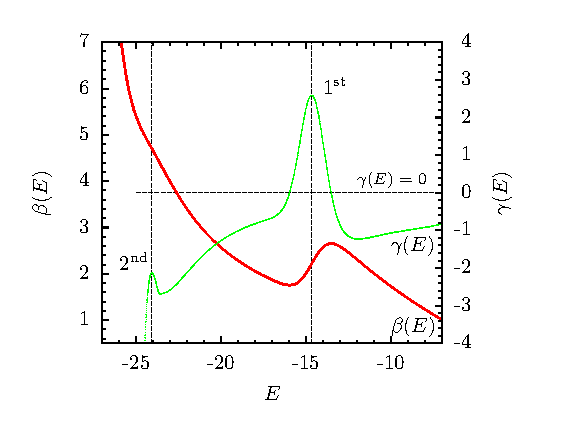
\includegraphics[width = 0.7\textwidth]{chapter2Figs/MicroAnalysisExample.eps}
\caption{\label{fig:Fig_1}%
Microcanonical inflection-point analysis of the inverse microcanonical temperature $\beta(E)$. The prominent back-bending region in $\beta(E)$, together with the positive-valued peak in its energy derivative $\gamma(E)$ at $E \approx -15$, indicates a \textit{first-order} transition. The negative-valued peak at $E\approx -24$ corresponds to a \textit{second-order} transition.}
\end{figure}
%

Alternatively, in the case of \textit{first-order} transitions, the transition temperature $\beta_{\mathrm{tr}}$ can be obtained by the means of the Maxwell construction, which was originally introduced to repair the unphysical back-bending in the pressure versus volume phase diagram for the van der Waals gas. However, in mesoscopic systems, finite-size effects lead to entropic suppression of the transition states, which is manifested in the backbending of $\beta(E)$ and the convex intruder in $S(E)$. 
%
\begin{figure}
\center
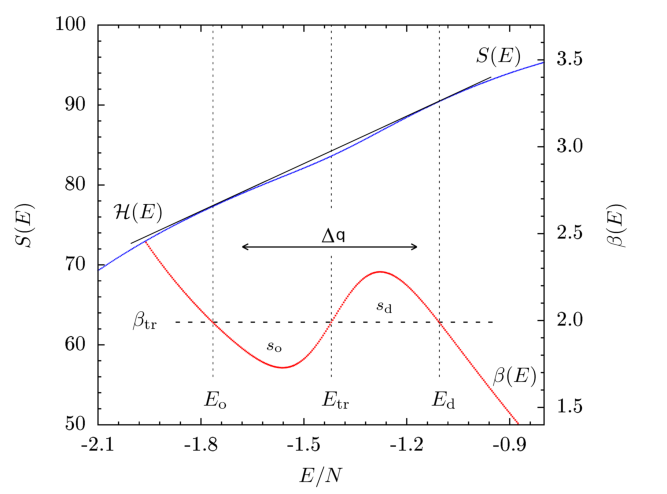
\includegraphics[width = 0.7\textwidth]{chapter2Figs/maxwellConstruct.pdf}
\caption{\label{fig:Fig_2}%
The convex region of the microcanonical entropy $S(E)$ and the back-bending of the microcanonical inverse temperature $\beta(E)$ are prominent indicators of \textit{first-order} transitions. The slope of the double-tangent Gibbs hull $\mathcal{H}(E)$ defines the transition temperature $\beta_{\mathrm{tr}}$. The Maxwell construction, defined by equal areas of $s_{\mathrm{o}}$ and $s_{\mathrm{d}}$, is itself positioned at $\beta_{\mathrm{tr}}$. The transition energy $E_{\mathrm{tr}}$ indicates the location of the largest separation between $\mathcal{H}(E)$ and $S(E)$, which signifies maximal entropic suppression of the transition states. The latent heat $\Delta Q$ corresponds to the width of the transition region between $E_{\mathrm{d}}$ and $E_{\mathrm{o}}$.}
\end{figure}
%
Figure \ref{fig:Fig_2} shows an example of a Maxwell construction. Its position is determined by the equality of the areas $s_{\mathrm{o}}$ and $s_{\mathrm{d}}$. Often referred to as \textit{surface entropies}, $s_{\mathrm{o}}$ and $s_{\mathrm{d}}$ are defined in terms of the integrals
\begin{eqnarray}
s_{\mathrm{o}} &=& \int_{E_{\mathrm{o}}}^{E_{\mathrm{tr}}} dE \:\: (\beta_{\mathrm{tr}}-\beta(E)), \\
s_{\mathrm{d}} &=& \int_{E_{\mathrm{tr}}}^{E_{\mathrm{d}}} dE \:\: (\beta(E)-\beta_{\mathrm{tr}}).
\end{eqnarray}
There are three intersections between the Maxwell line and the inverse temperature at energies $E_{\mathrm{o}}$, $E_{\mathrm{tr}}$, and $E_{\mathrm{d}}$. The separation between the boundary energies of the ordered pseudophase $E_{\mathrm{o}}$ and the disordered pseudophase $E_{\mathrm{d}}$, corresponds to the latent heat $\Delta Q = E_{\mathrm{d}} - E_{\mathrm{o}}$. The transition energy $E_{\mathrm{tr}}$ indicates the location where the intermediate states experience maximal entropic suppression.
The slope of the double-tangent Gibbs construction, also shown in Figure \ref{fig:Fig_2}, provides yet another definition of $\beta_{\mathrm{tr}}$. As a function of energy, the Gibbs hull is defined as
\begin{equation}
\mathcal{H}(E) = S(E_{\mathrm{o}}) + \beta_{\mathrm{tr}}[E-E_{\mathrm{o}}],
\end{equation}
where $\beta_{\mathrm{tr}}$ can be expressed in terms of the energy and entropy differences between the ordered and disordered pseudophases as
\begin{equation}
\beta_{\mathrm{tr}} = \frac{S_{\mathrm{d}}-S_{\mathrm{o}}}{E_{\mathrm{d}}-E_{\mathrm{o}}} = \frac{\Delta S}{\Delta Q}.
\end{equation}
With the exception of composite multi-step transitions, characterized by additional oscillations in the back-bending region of $\beta(E)$, the transition temperatures obtained by the means of the Maxwell and Gibbs constructions are identical.

 Based on the principle of minimal sensitivity and Ehrenfest's original idea of characterizing the order of a transition by the free-energy derivative at which a discontinuity occurs, one can likewise introduce a hierarchy of higher-order transitions microcanonically.
 
 
\section{The canonical ensemble}
The canonical ensemble describes the behavior of a closed system in thermal equilibrium with a large external heat bath at a fixed temperature $T$. In analogy to the density of states in the microcanonical ensemble, the partition function $Z(T)$ contains all the essential information about the thermodynamic properties of the system under consideration. It can be defined directly as a Laplace transform\footnote{Here we assume that the system under investigation has discrete energy levels, which is always true in the context of computational studies. In the case of a continuous energy spectrum, the discrete sum is replaced by the integral $Z(T) = \int dE \:\:  g(E) e^{-\frac{E}{k_{\mathrm{B}}T}}$.} of the microcanical density of states $g(E)$
\begin{equation}
Z(T) = \sum g(E) e^{-\frac{E}{k_{\mathrm{B}}T}},
\end{equation}
where $T$ is the canonical heat bath temperature and $k_{\mathrm{B}}$ is the Boltzmann constant. While the condition of thermal equilibrium prohibits any net average energy transfer between the system and the heat bath, the system can gain or loose energy through constant fluctuations and dissipations. This leads to the well known temperature dependent Boltzmann distribution, where the probability for a given microstate $\mu$ is given by 
\begin{equation}
p(\mu) = \frac{1}{Z(T)}e^{-\frac{\mathcal{H}(\mu)}{k_{\mathrm{B}}T}},
\end{equation}
and $\mathcal{H}$ is the Hamiltonian of the system. The appropriate thermodynamic potential in the canonical ensemble is the Helmholtz free energy
\begin{equation}
F(T) = -k_{\mathrm{B}}T \: \mathrm{ln}\, Z.
\end{equation}
This quantity represents the energy available to perform work and can be used to obtain all other thermodynamic quantities by differentiation. The temperature derivative of the free energy defines the canonical entropy
\begin{equation}
S(T) = -\frac{\partial}{\partial T}F(T)\bigg|_{N,V},
\end{equation} 
which measures the amount of disorder in the system.
The internal energy $U$ is defined as a sum over all microstate energies weighted by the Boltzmann distribution  
\begin{equation}
U(T) = \frac{\sum_{\mu} \mathcal{H}(\mu)e^{-\frac{\mathcal{H}(\mu)}{k_{\mathrm{B}}T}}}{Z(T)} =  \frac{\sum_{E} E \, g(E) e^{-\frac{E}{k_{\mathrm{B}}T}}}{Z(T)}
\end{equation}
and represents the average energy of the system. Alternatively, the internal energy can be obtained by differentiating the free energy
\begin{equation}
U(T) = k_{\mathrm{B}}T^{2}\frac{\partial}{\partial T} \mathrm{ln} Z\bigg|_{N,V}
= -T^{2}\frac{\partial}{\partial T}\left(\frac{F}{T}\right)\bigg|_{N,V}.
\end{equation}
The amount of energy needed to increase the temperature of the system by one unit is given by the specific heat 
$C_{V}$, defined as a temperature derivative of the internal energy
\begin{equation}
C_{V}(T) = \frac{\partial}{dT}U(T)\bigg|_{N,V} = -T\frac{\partial^{2}}{\partial T^{2}}F(T)\bigg|_{N,V},
\end{equation}
or differentiating the third term in equation 2.20 we get
\begin{eqnarray}
C_{V}(T) &=&  \frac{\partial}{dT}\frac{\sum_{E} E \, g(E) e^{-\frac{E}{k_{\mathrm{B}}T}}}{Z(T)} = -\frac{1}{k_{\mathrm{B}}T^2}\frac{\partial}{\partial \beta}\frac{\sum_{E} E \, g(E) e^{-\beta E}}{\sum_{E}g(E) e^{-\beta E}} \nonumber \\
&=& \frac{1}{k_{\mathrm{B}}T^2} \left[\left(\frac{\sum_{E} E^{2} \, g(E)  e^{-\beta E}}{Z(T)}\right) - \left(\frac{\sum_{E} E \, g(E)  e^{-\beta E}}{Z(T)}\right)^{2}\right] \nonumber \\
&=& \frac{1}{k_{\mathrm{B}}T^2}\left(\left<E^{2}\right> - \left<E\right>^{2}\right),
\end{eqnarray}
where the last expression corresponds to the variance of the Boltzmann distribution. This result is of a profound physical importance, establishing the connection between the macroscopic response quantity $C_{V}$, and microscopic fluctuations.

\subsection{Canonical analysis of phase transitions} 




\section{Configurational density of states}
\section{Generalized ensembles}

\chapter{Computational Methods}
\section{Markov chain Monte Carlo}
\subsection{Master equation and detailed balance}
\subsection{Metropolis sampling}
\section{Generalized ensemble Monte Carlo}
\subsection{Parallel tempering}
\subsection{Multiple Gaussian modified ensemble}
\subsection{Histogram reweighting methods}
\subsection{Multicanonical sampling}
\section{Simple Monte Carlo updates}

\chapter{Coarse-grained Homopolymer Model}
\section{Flexible elastic homopolymer}
\section{Interacting homopolymers}

\chapter{Confinement Effects on Structural Transitions in Flexible Homopolymers}
\section{Introduction}
\section{Canonical analysis}
\section{Inflection-point analysis}
\section{Hyper-phase diagrams}

\chapter{Impact of Bonded Interactions on the Ground-State Geometries of Flexible Homopolymers}
\section{Structural order parameters}
\section{15-mer}
\section{55-mer}

\chapter{Aggregation of Flexible Elastic Homopolymers}
\section{Introduction}
\section{Microcanonical analysis}
\subsection{Subphases and subphase transitions}
\subsection{Missing subphases and translational entropy}
\subsection{Density effects on the latent heat}

\chapter{Summary and Outlook}










\begin{figure}
\centerline{[ You could put a picture here. ]}
\caption{Example of a figure.}
\end{figure}

\begin{table}
\caption{Example of a table.}
\centerline{[The contents of the table would go here.]}
\end{table}



%~~~~~~~~~~~~~~~~ Reference ~~~~~~~~~~~~~~~~~~%
\addcontentsline{toc}{chapter}{Bibliography}
\begin{thebibliography}{99}
        %%%%%%%%%%% CHAPTER 2 %%%%%%%%%%%%%%%%%%
\bibitem{Bachmann2014}
M.~Bachmann, \emph{Thermodynamics and Statistical Mechanics of
Macromolecular Systems}, (Cambridge University Press, Cambridge,
2014).
%
\bibitem{Rugh2001}
H.~H.~Rugh , Phys.\ Rev.~E \textbf{64},
055101 (2001).

%%%%%%%%%%% Microcanonical Ensemble %%%%%%%%%%%

\bibitem{Kardar2007}
M.~Kardar, \emph{Statistical Physics of Particles}, (Cambridge University Press, New York, 2007).
%
\bibitem{Pathria}
R.~K.~Pathria, and P.~D.~Beale, \emph{Statistical Mechanics}, (Elsevier, Oxford, 2011).
%
\bibitem{Sethna2006}
J.~P.~Sethna, \emph{Statistical Mechanics: Entropy, Order Parameters, and Complexity}, 
(Oxford University Press, New York, 2006).
%


%%%%%%%%%%% Microcanonical Analysis %%%%%%%%%%%%
\bibitem{Gross2001} 
D.~H.~E.~Gross, \emph{Microcanonical Thermodynamics}, (World Scientific, Singapore,  2001).
%
\bibitem{Stevenson}
P.~M.~Stevenson, Phys.\ Rev.~D \textbf{23}, 2916 (1981).
%
\bibitem{Schnabel2011}
S.~Schnabel, D.~T.\ Seaton, D.~P.\ Landau, and M.~Bachmann, Phys.\ Rev.~E
\textbf{84}, 011127 (2011). 
%


%%%%%%%%%%% Canonical Analysis %%%%%%%%%%%%%%%%

\bibitem{Landau2000}
D.~P.\ Landau, and K.~Binder, \emph{A Guide to Monte Carlo Simulations in Statistical Physics}, (Cambridge University Press, Cambridge, 2000).

%%%%%%%%%%% Definitions of Density of States %%%%%%%%%

\bibitem{Calvo1995}
F.~Calvo, and P.~Labastie,  Chem.\ Phys.\ Lett. \textbf{247}, 395 (1995).
%




\end{thebibliography}


\end{document}


